\documentclass[12pt,a4paper]{article}
\usepackage{ctex}
\usepackage{amsmath,amscd,amsbsy,amssymb,latexsym,url,bm,amsthm}
\usepackage{epsfig,graphicx,subfigure}
\usepackage{enumitem,balance}
\usepackage{wrapfig}
\usepackage{mathrsfs,euscript}
\usepackage[usenames]{xcolor}
\usepackage{hyperref}
\usepackage[vlined,ruled,linesnumbered]{algorithm2e}
\hypersetup{colorlinks=true,linkcolor=black}

\newtheorem{theorem}{Theorem}
\newtheorem{lemma}[theorem]{Lemma}
\newtheorem{proposition}[theorem]{Proposition}
\newtheorem{corollary}[theorem]{Corollary}
\newtheorem{exercise}{Exercise}
\newtheorem*{solution}{Solution}
\newtheorem{definition}{Definition}
\newtheorem*{ndefinition}{Definition}
\newtheorem*{observation}{Observation}
\newtheorem*{conclusion}{Conclusion}
\theoremstyle{definition}

\renewcommand{\thefootnote}{\fnsymbol{footnote}}

\newcommand{\postscript}[2]
 {\setlength{\epsfxsize}{#2\hsize}
  \centerline{\epsfbox{#1}}}

\renewcommand{\baselinestretch}{1.0}

\setlength{\oddsidemargin}{-0.365in}
\setlength{\evensidemargin}{-0.365in}
\setlength{\topmargin}{-0.3in}
\setlength{\headheight}{0in}
\setlength{\headsep}{0in}
\setlength{\textheight}{10.1in}
\setlength{\textwidth}{7in}
\makeatletter \renewenvironment{proof}[1][Proof] {\par\pushQED{\qed}\normalfont\topsep6\p@\@plus6\p@\relax\trivlist\item[\hskip\labelsep\bfseries#1\@addpunct{.}]\ignorespaces}{\popQED\endtrivlist\@endpefalse} \makeatother
\makeatletter
\renewenvironment{solution}[1][Solution] {\par\pushQED{\qed}\normalfont\topsep6\p@\@plus6\p@\relax\trivlist\item[\hskip\labelsep\bfseries#1\@addpunct{.}]\ignorespaces}{\popQED\endtrivlist\@endpefalse} \makeatother

\begin{document}
\noindent

%========================================================================
\noindent\framebox[\linewidth]{\shortstack[c]{
\Large{\textbf{Lab03-GreedyStrategy}}\vspace{1mm}\\
CS214-Algorithm and Complexity, Xiaofeng Gao, Spring 2020.}}
\begin{center}
\footnotesize{\color{red}$*$ If there is any problem, please contact TA Shuodian Yu.}

% Please write down your name, student id and email.
\footnotesize{\color{blue}$*$ Name:Hongjie Fang  \quad Student ID:518030910150 \quad Email: galaxies@sjtu.edu.cn}
\end{center}

\begin{enumerate}
    \item
    There are $n+1$ people, each with two attributes $(a_i,b_i), i\in[0,n] \text{ and } a_i>1$. The $i$-th person can get money worth $c_i = \frac{\prod_{j=0}^{i-1}{a_j}}{b_i}$. We do not want anyone to get too much. Thus, please design a strategy to sort people from $1$ to $n$, such that the maximum earned money $c_{max}=\max\limits_{1\leq i\leq n} c_i$ is minimized. (Note: the 0-th person doesn't enroll in the sorting process, but $a_0$ always works for each $c_i$.)
    \begin{enumerate}
        \item Please design an algorithm based on greedy strategy to solve the above problem. (Write a pseudo code)
        \item Prove your algorithm is optimal.
    \end{enumerate}

   \begin{solution} The answers to the problems are as follows.
   \begin{enumerate}
   \item Sorting the people from $1$ to $n$ according to the products of their attributes $a_i \cdot b_i$ in a non-decreasing order. The pseudo code of calculate the minimized value of the maximum earned money $c_{max}$ is as follows (Alg.~\ref{Greedy-1}).

       \begin{minipage}[t]{0.8\textwidth}
        \begin{algorithm}[H]
            \KwIn{The array of people's attributes $a[0,\cdots,n], b[0,\cdots,n]$}
            \KwOut{The minimized value of the maximum earned money $c_{max}=\max\limits_{1\leq i\leq n} c[i]$, where $c[i] = \frac{\prod_{j=0}^{i-1}{a[j]}}{b[i]}$.}

            \BlankLine
            \caption{Greedy algorithm to minimize the maximum earned money}
            \label{Greedy-1}
            Sort people from $1$ to $n$ according to the products of their attributes $a[i] \cdot b[i]$ in a non-decreasing order.

            $cur \leftarrow a[0]$; $ans \leftarrow 0$;

            \For{$i = 1$ \textbf{to} $n$} {
                $c[i] \leftarrow cur / b[i]$;

                \If{$c[i] > ans$} {
                    $ans \leftarrow c[i]$;
                }
                $cur \leftarrow cur \cdot a[i]$;
            }
            \Return{$ans$};
        \end{algorithm}
        \end{minipage}
   \item Here we are going to prove that the result of the greedy algorithm to minimize the maximum earned money (Alg.~\ref{Greedy-1}) is optimal.
         \begin{ndefinition}[inversion]
         Given a sorting strategy $S$, after sorting according to $S$, an inversion is a pair of persons $i$ and $j$ such that $i < j$ but $a_i \cdot b_i > a_j \cdot b_j$.
         \end{ndefinition}
         \begin{observation}
         The sorting strategy in the greedy algorithm (Alg.~\ref{Greedy-1}) $S$ has no inversions. And a sorting strategy that has no inversions must be a result of the sorting strategy in the greedy algorithm (Alg.~\ref{Greedy-1}).
         \end{observation}
         \begin{observation}
         If a sorting strategy $S'$ has an inversion after sorting, it has one with a pair of consecutive, inverted persons after sorting.
         \end{observation}
         The correctness of these observations is obvious, so we do not discuss further here. Here we propose an important lemma as follows.
         \begin{lemma}\label{lemma1}
         Swapping two consecutive, inverted persons $i\ (1 \leq i < n)$ and $(i+1)$ reduces the number of inversions by one and does not increase the maximum earned money.
         \end{lemma}
         \begin{proof}
         Let $k$ be $\prod_{j=0}^{i-1}{a_j}$, then obviously $k$ is greater than $1$. Let $c_i\ (1 \leq i \leq n)$ be the original earned money of person $i$, and $c'_i$ be the earned money of person $i$ after swapping two consecutive, inverted persons $i$ and $(i+1)$. Originally, we have:
         \begin{displaymath}
         c_i = \frac{k}{b_i}, \quad c_{i+1} = \frac{ka_i}{b_{i+1}}.
         \end{displaymath}
         After swapping, we have:
         \begin{displaymath}
         c'_i = \frac{ka_{i+1}}{b_i}, \quad c'_{i+1} = \frac{k}{b_{i+1}}.
         \end{displaymath}
         Notice that $c_{i+1} > c'_{i+1}$ since $\frac{c_{i+1}}{c'_{i+1}} = a_i > 1$. Another important fact is that $c_{i+1} > c'_i$ because of the inverted pair's property of $a_i\cdot b_i > a_{i+1}\cdot b_{i+1}$. Hence,
         \begin{equation}
         \max(c'_i, c'_{i+1}) < c_{i+1} \leq \max(c_i, c_{i+1}).
         \label{eq1-1}
         \end{equation}
         Notice that the swapping of person $i$ and $(i+1)$ does not change other person's earned money $c_j\ (1 \leq j \leq n, j \ne i, j\ne i+1)$, therefore combining with Equation \eqref{eq1-1} we have:
         \begin{equation}
         c'_{max} = \max\limits_{1\leq i\leq n} c'_i \leq \max\limits_{1\leq i\leq n} c_i = c_{max}.
         \label{eq1-2}
         \end{equation}
         Equation \eqref{eq1-2} shows that the swapping does not increase the maximum earned money. And it's obvious that the swapping reduces the number of inversions by one, since it has no effect on other persons. Therefore, swapping two consecutive, inverted persons $i\ (1 \leq i < n)$ and $(i+1)$ reduces the number of inversions by one and does not increase the maximum earned money.
         \end{proof}
         With Lemma \ref{lemma1} we can easily prove the optimality of the greedy algorithm (Alg.~\ref{Greedy-1}).
         \begin{theorem}
         The sorting strategy of the greedy algorithm (Alg.~\ref{Greedy-1}) is optimal.
         \end{theorem}
         \begin{proof}
         Define $S$ to be an optimal schedule that has the fewest number of inversions.
         \begin{itemize}
         \item If $S$ has no inversions, then according to our observations, $S$ must be a result of the sorting strategy in the greedy algorithm. Therefore, the sorting strategy of the greedy algorithm is optimal.
         \item If $S$ has an inversion, let the pair of persons $i$ and $(i+1)$ be an adjacent inversion. According to Lemma \ref{lemma1}, swapping persons $i$ and $(i+1)$ reduces the number of inversions by one and does not increase the maximum earned money. This contradicts the definition of $S$.
         \end{itemize}
         In conclusion, the sorting strategy of the greedy algorithm (Alg.~\ref{Greedy-1}) is optimal.
         \end{proof}
   \end{enumerate}
   \end{solution}
   \clearpage

    \item
    \textbf{Interval Scheduling} is a classic problem solved by greedy algorithm and we have introduced it in the lecture: given $n$ jobs and the $j$-th job starts at $s_j$ and finishes at $f_j$. Two jobs are compatible if they do not overlap. The goal is to find maximum subset of mutually compatible jobs. Tim wants to solve it by sort the jobs in descending order of $s_j$. Is this attempt correct? Prove the correctness of such idea, or else provide a counter-example.
   \begin{conclusion}
     This idea is correct.
   \end{conclusion}
   \begin{proof}
   Assume that in the following discussions, the sets of jobs are already sorted non-increasingly according to their starting time. For instance, a set of job $\{t_1, t_2, \cdots, t_p\}$ satisfies $s_{t_1} \geq s_{t_2} \geq \cdots \geq s_{t_p}$.

   Let $\{i_1, i_2, ..., i_k\}$ denote the set of jobs selected by this idea.

   Let $\{j_1, j_2, ..., j_m\}$ denote the set of jobs in an optimal solution with $i_1 = j_1, i_2 = j_2, \cdots, i_r = j_r$ for the largest possible value $r$. And it is obvious that $m \geq k$.
   \begin{itemize}
   \item \textbf{Case 1 ($r = k$):} If $m > k$, then there still are some jobs that can be chosen with this idea, since the jobs selected by this idea is also selected by the optimal solution and the optimal solution includes other jobs. And with this idea, we can not miss any jobs that can be chosen currently, therefore more than $k$ jobs must be selected finally. This contradicts the number of selected jobs by this idea is only $k$. Hence, we have $m = k$ and the jobs selected by this idea is exactly the same as the optimal solution. Thus, the idea will provide us an optimal solution.
   \item \textbf{Case 2 ($r < k$):} This situation is shown in Fig.~\ref{fig1} as follows.

    \begin{figure}[h]
    \centering
    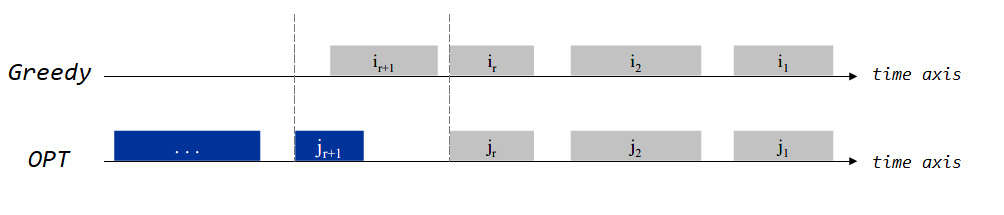
\includegraphics[width=6in]{problem2-explanation.png}
    \caption{The situation in Case 2 ($r < k$)}\label{fig1}
    \end{figure}

    When choosing the $(r+1)$-th job, the disagreements between the two solutions appear. With this idea, we choose job $i_{r+1}$; but in the optimal solution, we choose job $j_{r+1}$. Notice that we can substitute job $j_{r+1}$ with job $i_{r+1}$ in the optimal solution without loss of its optimality and it is a still feasible solution. This contradicts with the maximality of $r$.
   \end{itemize}
   In conclusion, this idea can provide us an optimal solution. Therefore it is correct.
   \end{proof}
   \clearpage

    \item
    There are $n$ lectures numbered from $1$ to $n$. Lecture $i$ has duration (course length) $t_i$ and will close on $d_i$-th day. That is, you could take lecture $i$ \textbf{continuously} for $t_i$ days and must finish before or on the $d_i$-th day. The goal is to find the maximal number of courses that can be taken. (Note: you will start learning at the $1$-st day.)

    Please design an algorithm based on greedy strategy to solve it. You could use the data structure learned on Data Structure course. You need to write pseudo code and prove its correctness.

   \begin{solution} The pseudo code of the greedy algorithm is as follows (Alg.~\ref{Greedy-2}).

        \begin{minipage}[t]{0.8\textwidth}
        \begin{algorithm}[H]
            \KwIn{The duration of every lecture $t[1,\cdots,n]$ and the deadline of every lecture $d[1,\cdots,n]$.}
            \KwOut{The maximum number of courses that can be taken.}

            \BlankLine
            \caption{Greedy algorithm to maximize the number of taken courses}
            \label{Greedy-2}
            Sort courses by their deadlines $d[i]$ in an non-descending order, if several courses has the same deadline, then sort them by their duration time $t[i]$ in an non-descending order.

            $time \leftarrow 1$;

            $taken \leftarrow \varnothing$; \quad \tcp{\color{blue}$taken$ can be implemented as a max-heap.}

            \For{$i = 1$ \textbf{to} $n$} {
               \If{$time + t[i] - 1 \leq d[i]$} {
                    $taken \leftarrow taken \cup \{t[i]\}$;

                    $time \leftarrow time + t[i]$;
               } \ElseIf {$taken \ne \varnothing$} {
                    $maxt \leftarrow \max\limits_{t' \in taken}{t'}$;

                    \If{$t[i] < maxt$} {
                        $taken \leftarrow (taken \backslash \{maxt\}) \cup \{t[i]\}$;

                        $time \leftarrow time - maxt + t[i]$;
                    }
                 }
            }
            \Return{$\mathrm{size}(taken)$};  \quad \tcp{\color{blue}size($s$) will return the size of set $s$.}
        \end{algorithm}
        \end{minipage}

        \textbf{\color{red}Explanation.} Let me explain the idea of the pseudo code explicitly. First we sort the courses by their deadlines in a non-descending order. Then we consider about every course in turn:
        \begin{itemize}
        \item If the current course can be taken (i.e., there is enough time to finish it before its deadline), then we will update the current finish $time$ of all taken courses and put the duration of current course into the $taken$ set, which means we are going to take it under the current circumstance.
        \item If the time is not enough for finishing the current course, then we compare the duration of the current course with the maximum duration in the $taken$ set.
        \begin{itemize}
        \item If the current course's duration is less than the maximum duration in the $taken$ set, then we will substitute the course which has the maximum duration in $taken$ set with the current course. Therefore we need to update the $taken$ set and the current finish $time$ of all taken courses.
        \item If the current course's duration isn't less than the maximum duration in the $taken$ set, then we won't take the current course.
        \end{itemize}
        \end{itemize}
        After considering every course, the size of the $taken$ set is the maximum number of courses that can be taken.

        \textbf{\color{red}Time Complexity Analysis.} Now let us analyze its time complexity first. We can use a \textbf{max-heap} to implement the $taken$ set, because it supports inserting elements, erasing the maximum element and query the maximum element in a time complexity of $O(\log{n})$, which perfectly fits our requirements. Therefore, both the time complexity of the sorting process and the time complexity of the selecting process are $O(n\log{n})$. Hence, the time complexity of the greedy algorithm is $O(n\log{n})$.

        \textbf{\color{red}Correctness Proof.} Define a solution $S$ as a set of courses that can be taken (i.e., a feasible answer). Let us propose some definitions and lemmas first.
        \begin{lemma}\label{lemma3-0}
        Given a solution $S$, we can arrange the order of the courses in $S$ as follows.
        \begin{itemize}
        \item Sort the courses by their deadlines $d_i$ in an non-descending order, and if several courses has the same deadline, then sort them by their duration $t_i$ in an non-descending order.
        \item Schedule the courses in turn with no idle time.
        \end{itemize}
        \end{lemma}
        \begin{proof}
        According to the content of the lecture, we know that this method can minimize the maximum of delay time.
        Since solution $S$ is a feasible answer, which means the minimum of maximum delay time is 0, it is obviously a feasible method to arrange the courses.
        \end{proof}
        {\color{blue} In the following discussion, given a solution $S$ and we will schedule the courses in $S$ with the methods in Lemma 3.}
        \begin{ndefinition}[a reversed pair]
        If two courses $i$ and $j$ satisfying $d_i \leq d_j$, $t_i > t_j$ and course $i$ is in solution $S$ while course $j$ is not, then we call them a reversed pair $(i,j)$ in solution $S$.
        \end{ndefinition}

        \begin{lemma}
        \label{lemma3-1}
        Our greedy algorithm's solution $S$ has no reversed pairs.
        \end{lemma}
        \begin{proof}
        Let us prove it by contradiction. Suppose there exists a reversed pair $(i,j)$ in solution $S$ provided by our greedy algorithm.
        \begin{itemize}
        \item First, course $j$ must be considered after course $i$ owing to the property that $d_i \leq d_j$ and $t_i > t_j$. After considering about course $j$, both course $i$ and course $j$ must be in our current $taken$ list.
        \begin{itemize}
        \item For course $i$, it won't appear on the solution's $taken$ list if it is not in our current $taken$ list, because we won't re-consider about the courses.
        \item For course $j$, if we have enough time to finish it, then it must be taken according to the algorithm. If we do not have enough time to finish it, we will search for a course which consumes more time than course $j$ in the $taken$ list. And there must exist at least one such course, since course $i$ is a feasible choice. Therefore, course $j$ must be substituted for another course and appear in the $taken$ list after considering about course $j$.
        \end{itemize}
        \item Second, if one of the two courses are replaced by another courses in the future, it will be course $i$. If there is a replacement in the future, we will consider about the course which has the longest duration time first. Since $t_i > t_j$, $i$ must be considered first. Therefore, if one of the two courses is replaced, then $i$ must be replaced first, which contradicts our premise that course $i$ is in solution $S$ while $j$ is not.
        \end{itemize}
        Therefore, our greedy algorithm's solution $S$ has no reversed pairs.
        \end{proof}
        \begin{lemma}
        \label{lemma3-2}
        If there is a reversed pair $(i,j)$ in the solution $S$, we can drop course $i$ and take course $j$ based on solution $S$ to form solution $S'$. Solution $S'$ is still a feasible answer and has the same number of courses as solution $S$. What's more, the number of reversed pair in $S'$ is strictly less than that in $S$.
        \end{lemma}
        \begin{proof}
        In solution $S'$, we drop the course $i$ so we have a continuous period of time of $t_i$ days. Course $j$ needs $t_j$ days and $t_j$ is less than $t_i$ according to the definition of the reversed pair, so we can schedule course $j$ in this continuous period of time of $t_i$ days. And we can finish course $j$ on time since the deadline of course $j$ is even later than the deadline of course $i$. Therefore, solution $S'$ is a feasible answer. And since we drop a course and take another course, the number of courses will not change, that is, solution $S'$ has the same number of courses as solution $S$.

        Every reversed pair in solution $S'$ can map to a reversed pair in solution $S$. If the pair does not involve course $i$ and course $j$, then it's obviously true - we can map the pair to itself in solution $S$. If there is a pair of reversed courses involving course $j$ or course $i$, then there are two cases as follows. Suppose another involved course is course $k$.
        \begin{itemize}
        \item \textbf{Case 1:} $(j,k)$ is a reversed pair in solution $S'$, which means $t_j > t_k$, $d_j < d_k$ and course $j$ is taken while course $k$ is not taken in solution $S'$. Then in solution $S$, $(i,k)$ must be a reversed pair, since $t_i > t_j > t_k$ and $d_i < d_j < d_k$. Then we can map the reversed pair $(j,k)$ in solution $S'$ to the reversed pair $(i,k)$ in solution $S$.
        \item \textbf{Case 2:} $(k,i)$ is a reversed pair in solution $S'$, which means $t_k > t_i$, $d_k < d_i$ and course $k$ is taken while course $i$ is not taken in solution $S'$. Then in solution $S$, $(k,j)$ must be a reversed pair, since $t_k > t_i > t_j$ and $d_k < d_i < d_j$. Then we can map the reversed pair $(k,i)$ in solution $S'$ to the reversed pair $(i,k)$ in solution $S$.
        \end{itemize}
        Therefore, we construct a injection from the reversed pair in solution $S'$ to solution. Hence, we can come to a conclusion that the number of reversed pair in solution $S'$ is no more than that in solution $S$. Notice that we the reversed pair $(i,j)$ in solution $S$ disappears in solution $S'$, so the number of reversed pair in solution $S'$ is strictly less than that in solution $S$.
        \end{proof}
        \begin{theorem}
        Our greedy algorithm's solution $S$ is optimal.
        \end{theorem}
        \begin{proof}
        Suppose there is an optimal solution $S'$, we are able to transform it to a solution with no reversed pairs without changing its number of courses by repeating the steps. The definition of a step is as follows.
        \begin{itemize}
        \item Check if there is a reversed pair in solution $S'$. If false, the process is finished.
        \item If true, choose a reversed pair in $S'$ called $(i,j)$. Then drop course $i$ and take course $j$ based on solution $S'$ to form a new solution $S''$. Assign $S''$ to $S'$.
        \end{itemize}
        According to Lemma \ref{lemma3-2}, the solution $S'$ after transforming is still a feasible solution with the same number of courses (i.e., without loss of optimality). Since every time we reduce the number of reversed pair in solution $S'$ and the number of reversed pair cannot be less than 0, the process will end in finite steps. Therefore, {\color{blue}there exists an optimal solution with no reversed pairs}.

        Assume that in the following discussions, the sets of taken courses are already sorted non-decreasingly according to their deadlines. And we assign new indexes from $1$ to $n$ to the courses according to the sorting result. Thus, two courses indexed $i$ and $j$ satisfying $i < j$ indicates that $d_i < d_j$ or $d_i = d_j$ and $t_i \leq t_j$.

        Let $\{i_1, i_2, ..., i_k\}$ denote the set of taken courses in greedy algorithm's solution $S$.

        Let $\{j_1, j_2, ..., j_m\}$ denote the set of taken courses in a \textbf{no-reversed-pair optimal} solution $S'$ which has the \textbf{most number of courses overlapped} with solution $S$, and obviously we have $m \geq k$. Let $r$ be the number of courses that solution $S'$ is overlapped with solution $S$. We are going to prove that $S$ is
        exactly the same solution as $S'$.
        \begin{itemize}
        \item \textbf{Case 1 ($r = k$):} If $m = k$, then the solution $S$ is exactly the same as solution $S'$.

            If $m > k$, then all the courses taken in solution $S$ must be taken in solution $S'$. Suppose the first course in solution $S'$ which is not taken in solution $S$ is $i$ and $i$ must satisfy $i \leq j_{k+1}$ because of $m > k$.
            \begin{itemize}
            \item \textbf{Case 1.1 (Fig.~\ref{fig11}):} If $i = j_{k+1}$, then in greedy algorithm we are able to find that course $i$ can be taken, which contradicts the premise that the solution $S'$ of greedy algorithm contains only $k$ courses.
            \begin{figure}[h]
            \centering
            % Requires \usepackage{graphicx}
            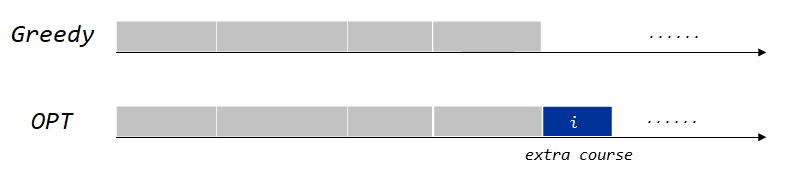
\includegraphics[width=4.2in]{problem3-case1-1.png}\\
            \caption{The situation of Case 1.1}\label{fig11}
            \end{figure}
            \item \textbf{Case 1.2 (Fig.~\ref{fig120}):} If $i = j_p\ (1 \leq p \leq k)$, then according to the optimal solution $S'$, we know that when we are considering course $i$ in greedy algorithm, we can put course $i$ into the $taken$ set. But somehow course $i$ is replaced by another course, say course $i'$, satisfying $i' > i$ and $t_{i'} < t_i$. Under some circumstances, course $i'$ may be replaced by another course, say course $i''$, satisfying $i'' > i' > i$ and $t_{i''} < t_{i'} < t_i$. Repeat the process until we find the first course that is still in solution $S$ called $i^*$ (Fig.~\ref{fig3}), and we know that $i^* > i$ and $t_{i^*} < t_i$. Then course $i^*$ must in the solution $S'$ since every course in solution $S$ is in solution $S'$. Therefore, there exists a reversed pair $(i, i^*)$ in solution $S'$, which contradicts the premise that $S'$ is a no-reversed-pair solution.
            \begin{figure}[h]
            \centering
            % Requires \usepackage{graphicx}
            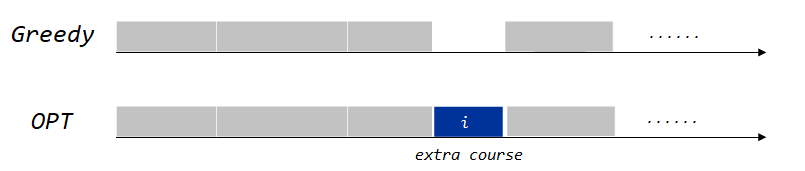
\includegraphics[width=4.2in]{problem3-case1-2-0.png}\\
            \caption{The situation of Case 1.2}\label{fig120}
            \end{figure}
            \begin{figure}[h]
            \centering
            % Requires \usepackage{graphicx}
            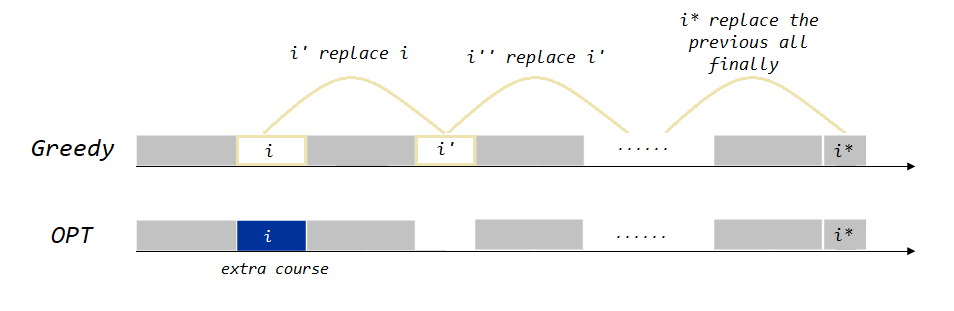
\includegraphics[width=4.5in]{problem3-case1-2-1.png}\\
            \caption{The replacing relations of Case 1.2}\label{fig3}
            \end{figure}
            \end{itemize}
        \item \textbf{Case 2 ($r < k$):} There exists an earliest course which is taken in solution $S$ but is not taken in solution $S'$, say $i$, and there exists an earliest course which is taken in $S'$ but is not taken in solution $S$, say $j$ (here earliest means smallest-index).
        \begin{itemize}
            \item \textbf{Case 2.1 ($d_i \geq d_j$ and $t_i = t_j$) (Fig.~\ref{fig21}):} Since the deadline of course $i$ is even later than the deadline of course $j$, we can drop course $j$ and take course $i$ in solution $S'$ to form a new no-reversed-pair solution $S^*$,
            which has $(r+1)$ overlapped course with $S$, and that contradicts the maximality of $r$.
            \begin{figure}[h]
            \centering
            % Requires \usepackage{graphicx}
            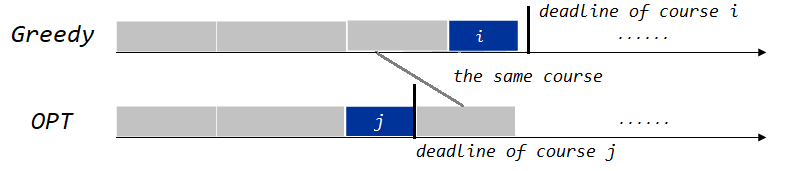
\includegraphics[width=4.2in]{problem3-case2-1.png}\\
            \caption{The replacing relations of Case 2.1}\label{fig21}
            \end{figure}
            \item \textbf{Case 2.2 ($d_i \geq d_j$ and $t_i < t_j$):} $(j, i)$ is a reversed pair in solution $S'$, which contradicts the premise that $S'$ is a no-reversed-pair solution.
            \item \textbf{Case 2.3 ($d_i \geq d_j$ and $t_i > t_j$) (Fig.~\ref{fig23}):} In greedy algorithm, we will consider about course $j$ first. According to the solution $S'$ we know that $j$ must be put
            into $taken$ set after considering about it. If there is a replacement in the future, we will consider about the course which has the longest duration time first.
            Since $t_i > t_j$, $i$ must be considered first. Therefore, it one of the two courses is replaced, then $i$ must be replaced first, which contradicts our premise
            that course $i$ is taken in solution $S$ while $j$ is not taken in solution $S$.
            \begin{figure}[h]
            \centering
            % Requires \usepackage{graphicx}
            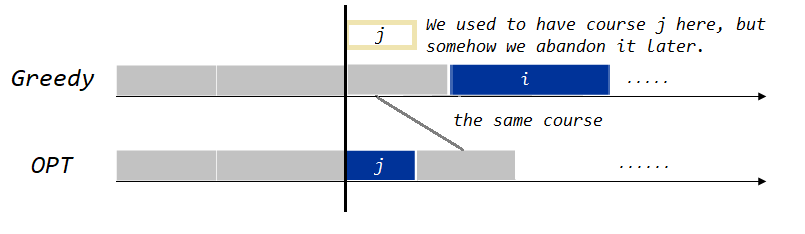
\includegraphics[width=4.2in]{problem3-case2-3.png}\\
            \caption{The replacing relations of Case 2.3}\label{fig23}
            \end{figure}
            \item \textbf{Case 2.4 ($d_i < d_j$ and $t_i > t_j$):} $(i, j)$ is a reversed pair in solution $S$, which contradicts with Lemma \ref{lemma3-1}.

            \item \textbf{Case 2.5 ($d_i < d_j$ and $t_i \leq t_j$) (Fig.~\ref{fig4}):} We can drop course $j$ and take course $i$ in solution $S'$ to form a new no-reversed-pair solution $S^*$.
            Notice that we can shift the course in $S'$ between $i$ and $j$ towards right, since they are corresponded with the course in $S$. Therefore, we can drop the course $j$
            and take course $i$ in exactly the same place as solution $S$. Therefore, $S^*$ has $(r+1)$ overlapped course with $S$, and that contradicts the maximality of $r$.
            \begin{figure}[h]
              \centering
              % Requires \usepackage{graphicx}
              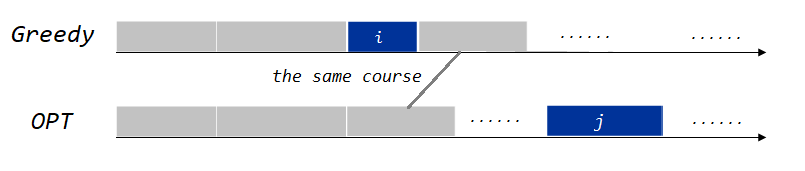
\includegraphics[width=4in]{problem3-case2-5.png}\\
              \caption{The situation of Case 2.5}\label{fig4}
            \end{figure}
        \end{itemize}
        \end{itemize}
        In summary, solution $S$ is exactly the same solution as $S'$. Therefore, solution $S$ is optimal.
        \end{proof}
     Therefore, we prove that our greedy algorithm is optimal.
   \end{solution}
    \item
    Let $S_1,S_2,\dots,S_n$ be a partition of $S$ and $k_1,k_2,\dots,k_n$ be positive integers. Let $\mathcal{I}=\{I: I \subseteq S,|I \cap S_i| \leq k_i \text { for all } 1 \leq i \leq n\}$. Prove that $\mathcal{M}=(S,\mathcal{I})$ is a matroid.

   \begin{proof} A matroid should satisfy two requirements: hereditary and exchange property. We prove them respectively as follows.
       \begin{itemize}
       \item (\textbf{Hereditary}) Suppose $I \in \mathcal{I}$ and $I' \subseteq I$. On one hand, since $I$ is a subset of $S$, $I'$ is a surely subset of $S$, that is, $I' \subseteq S$. On the other hand, for all $i$ in range $[1,n]$, we have $(I' \cap S_i) \subseteq (I \cap S_i)$, therefore, $|I' \cap S_i| \leq |I \cap S_i| \leq k_i$. Hence, we can draw the conclusion that $I' \in \mathcal{I}$. Therefore, $\mathcal{I}$ is hereditary and $\mathcal{M}=(S,\mathcal{I})$ is an independent system.
       \item (\textbf{Exchange Property}) Suppose $I \in \mathcal{I}$, $I' \in \mathcal{I}$ and $|I| < |I'|$. Since $S_1, S_2,\cdots,S_n$ is a partition of $S$, we can draw the following simple conclusions (Eqn.~\eqref{eq4-1}).
           \begin{equation}
           \begin{aligned}
           \cup_{i=1}^n (I \cap S_i) = I,& \quad \cup_{i=1}^n (I' \cap S_i) = I',\\
           (I \cap S_i) \cap (I \cap S_j) = \varnothing,& \quad (I' \cap S_i) \cap (I' \cap S_j) = \varnothing.
           \end{aligned}
           \label{eq4-1}
           \end{equation}
           Therefore, the following formulas (Eqn.~\eqref{eq4-2}) can be derived.
           \begin{equation}
           |I| = \sum_{i=1}^n |I \cap S_i|,\quad |I'| = \sum_{i=1}^n |I' \cap S_i|
           \label{eq4-2}
           \end{equation}
           Since $|I| < |I'|$, there exists an index $i^*$ in range $[1,n]$ such that $|I \cap S_{i^*}| < |I' \cap S_{i^*}| \leq k_i$.

           Therefore, there exists an element $x$ satisfying $x \in I' \cap S_{i^*}$ and $x \notin I \cap S_{i^*}$, which indicate that $x \in I' \backslash I$. Let $I^*$ be $I \cup \{x\}$, then
           \begin{itemize}
           \item For all the indexes $i$ satisfying $1 \leq i \leq n$ and $i \ne i^*$, we have $I^* \cap S_i = I \cap S_i$, therefore,
           \begin{displaymath}
           |I^* \cap S_i| = |I \cap S_i| \leq k_i
           \end{displaymath}
           \item For index $i^*$, we have $I^* \cap S_{i^*} = (I \cap S_{i^*}) \cup \{x\}$, therefore,
           \begin{displaymath}
           |I^* \cap S_{i^*}| = |I \cap S_{i^*}| + 1 \leq |I' \cap S_{i^*}| \leq k_{i^*}
           \end{displaymath}
           \end{itemize}
           In summary, we can derive that $I^* \in \mathcal{I}$. Therefore, $\mathcal{M}=(S,\mathcal{I})$ satisfies the exchange property.
       \end{itemize}
       In conclusion, $\mathcal{M}=(S,\mathcal{I})$ is a matroid.
   \end{proof}
\end{enumerate}

\vspace{20pt}

\textbf{Remark:} You need to include your .pdf and .tex files in your uploaded .rar or .zip file.

%========================================================================
\end{document}
